
 \documentclass[12pt]{article} % Документ принадлежит классу article, а также будет печататься в 12 пунктов.
\usepackage[russian]{babel} % Пакет поддержки русского языка
\usepackage{amsmath} %пакет формул
\title{Теория Алгоритма} % Заглавие документа
\usepackage{alltt}
\date{\today} % Дата создания
\parindent=1cm
\usepackage{graphicx}
\usepackage{amsfonts} 
\graphicspath{{pictures/}}
\DeclareGraphicsExtensions{.png}

\pdfinfo{
	/Author (Lemanskiy Konstantin Yurevich)
	/Title  (numerical methods)
	/CreationDate (D:20040502195600)
	/Subject (PDFLaTeX)
	/Keywords ()
}
 \begin{document}
 	
 		\section{Интерполяция сеточных функций с помощи многочленов Лагранжа}
 		\[L_k(x) = \sum_{i=0}^{i=k}\;\left( \prod_{0 \geq j \geq i,\, j \neq i} \cfrac{(x - x_j)}{x_i - x_j} \right) f_i \]
 		Пример для $(x_1, y_1), (x_2, y_2)$:
 		\[L_2(x) = \cfrac{(x - x_2)}{(x_1 - x_2)} y_1 + \cfrac{(x - x_1)}{(x_2 - x_1)} y_2 \]
 		Добавим еще одну точку $(x_1, y_1), (x_2, y_2), (x_3, y_3)$:
 		\[L_3(x) = \cfrac{(x - x_2)(x - x_3)}{(x_1 - x_2)(x_1 - x_3)} y_1 + \cfrac{(x - x_1)(x - x_3)}{(x_2 - x_1)(x_2 - x_3} y_2  + \cfrac{(x - x_1)(x - x_2)}{(x_3 - x_1)(x_3 - x_2)} y_3 \]
 		Пример:
 		\begin{verbatim}
 			from interpolation.inter_net_func import *
 			from interpolation.ploting import plot_result
 			
	 		x_arr = [1, 2, 5, 10]
	 		y_arr = [2, 4, -7, 2]
	 		plot_result(x_arr, y_arr, LagrangeExpr(x_arr, y_arr))
 		\end{verbatim}
 		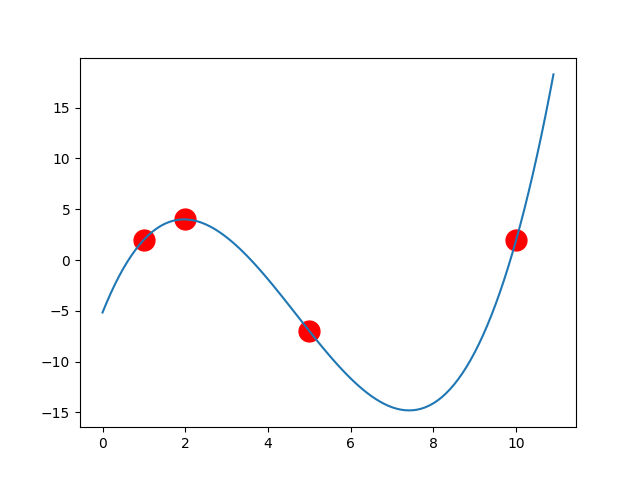
\includegraphics{1}
 		Пример2:
 		\begin{verbatim}
 			from interpolation.inter_net_func import *
 			from interpolation.ploting import plot_result
 			
 			x_arr = [1, 2, 5, 7,  10]
 			y_arr = [2, 4, -7, 10,  2]
 			plot_result(x_arr, y_arr, LagrangeExpr(x_arr, y_arr))
 		\end{verbatim}
 		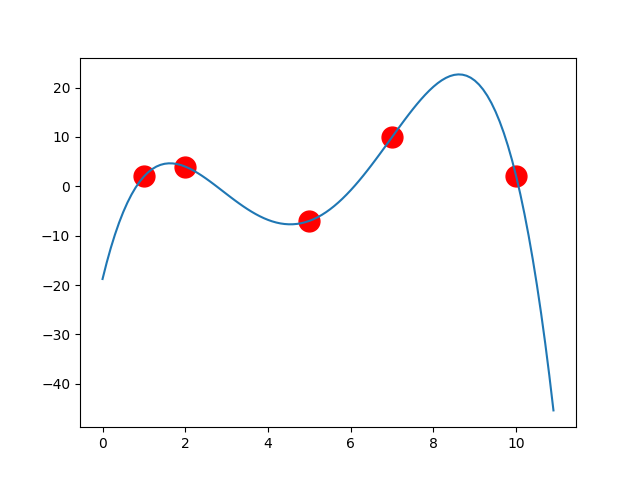
\includegraphics{2}
 		\section{Интерполяция сеточных функций с помощи многочленов Ньютона}
 		На бумаге многочлен ньютона можно опимсать так:
 		\[N_k(x) = a_0 + a_1(x-x_1) + a_2(x-x_1)(x-x_2) + \dots + a_{k-1} \prod_{i=1}^{i=k-1}(x - x_i)\]
 		где $a_k$ это переменные, которые можно найти из соответствующих ур-ий:
 		\[ \begin{cases}
 			y_1 = a_0\\
 			y_2 = a_0 + a_1(x_2-x_1)\\
 			y_3 = a_0 + a_1(x_3-x_1) + a_2(x_3-x_1)(x_3-x_2)\\
 			\dots
 		\end{cases}\]
 		Пример:
 		\begin{tabbing}
 			MMM \= MMM \kill
 		\textbf{x} \> \textbf{y}\\
 			1 \> 4\\
 			3 \> 5 \\
 			4 \> 7 \\
		\end{tabbing}
		\[ N_3(x) = a_0 + a_1(x-x_1) + a_2(x-x_1)(x-x_2)  \]
		\[N_3(x) = a_0 + a_1(x-1) + a_2(x-1)(x-3)\]
		\[ \begin{cases}
			y_1 = a_0\\
			y_2 = a_0 + a_1(x_2-1)\\
			y_3 = a_0 + a_1(x_3-1) + a_2(x_3-1)(x_3-3)\\
		\end{cases} \]
		\[ \begin{cases}
			a_0 = 4\\
			a_1 = \cfrac{y_2-a_0}{(x_2-1)} = \cfrac{5-4}{(3-1)} = 0.5\\
			a_2 = \cfrac{y_3 - a_0 - a_1(x_3-1)}{(x_3-1)(x_3-3)} = \cfrac{7 - 4 - 0.5(4-1)}{(4-1)(4-3)} = 0.5 \\
		\end{cases} \]
		\[N_3(x) = 4 + 0.5(x-1) + 0.5(x-1)(x-3)\]
		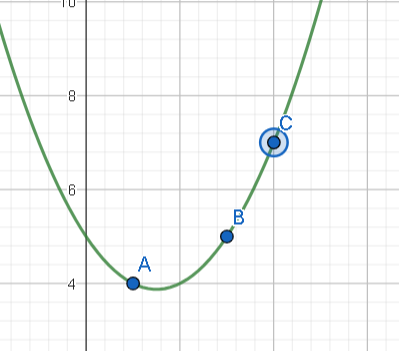
\includegraphics{3}
		И человеку было удобно так решать, но удобно не значит просто. Поэтому решили найти методы вычислять коофиценты быстрее.\\
		Добавим некоторые сущности:
		\[f(x_i, x_{i+1}) = \cfrac{y_{i+1} - y_i}{x_{i+1} - x_i} \]
		\[f(x_i, x_{i+1}, x_{i+2}) = \cfrac{f(x_{i+1}, x_{i+2}) - f(x_i, x_{i+1})}{x_{i+2} - x_i} \]
		\[f(x_i, x_{i+1},\dots , x_{i+k}) = \cfrac{f(x_{i+1}, x_{i+2}, \dots,  x_{i+k}) - f(x_i, x_{i+1}, \dots, x_{i+k})}{x_{i+k} - x_i} \]
		И тогда обобщенная формула ньютона выглядит так:
		\[N_k(x) = y_1 + f(x_1, x_{2})(x-x_1) + f(x_1, x_2, x_3)(x-x_1)(x-x_2) + \dots + f(x_1, x_{2},\dots , x_{k}) \prod_{i=1}^{i=k-1}(x - x_i)\]
		Проверим что это так:
		\[ \begin{cases}
			a_0 = 4\\
			a_1 = f(x_1, x_2) = \cfrac{5 - 4}{3 - 1} = 0.5\\
			a_2 = f(x_1, x_2, x_3) = \cfrac{ \cfrac{y_3 - y_2}{x_3 - x_2} - 0.5}{4-1} =  \cfrac{ 2 - 0.5}{4-1} = 0.5 \\
		\end{cases}\]
		Как видим результат аналогичный.\\
		Итак мы смогли структуризировать вычисления, но как их упростить? Рассмотрим задачу когда точки лежат на сетке с равным интервалом те $x_{i + 1} = x_i + h$:
		\[f(x_i, x_{i + 1}, x_{i + 2}, \dots , x_{i + k}) = \cfrac{\sum_{j=0}^{k} (-1) ^ j C_k^j y_{i+j}}{k!h^k}\]
		Что-ж мы еще чуть чуть упростили вычисления, но они все равно ужастно сложные. Зачем же тогда нужен этот метод? Попробуем добавить точку (2, 7):
		 \[N_4(x) = a_0 + a_1(x-1) + a_2(x-1)(x-3) + a_3(x-1)(x-3)(x-4)\]
		 И если попробовать вычислить $a_0, a_1, a_2$ окажутся аналогичными, а $a_3$: \[ a_3 =  \cfrac{y_4 - a_0 - a_1(x_4-1) - a_2(x_4-1)(x_4-3)}{(x_4-1)(x_4-3)(x_4-4)} = \cfrac{7 - 4 - 0.5(2-1) - 0.5(2-1)(2-3)}{(2-1)(2-3)(2-4)} = 1.5 \]
		 \[N_4(x) = 4 + 0.5(x-1) + 0.5(x-1)(x-3) + 1.5(x-1)(x-3)(x-4)\]
		 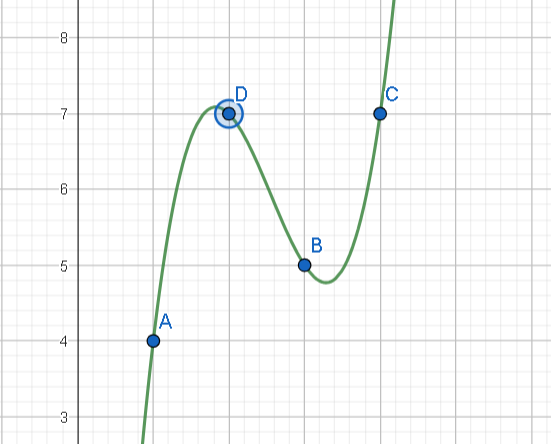
\includegraphics{4}
		 Пример работы алгоритма:
		 \begin{verbatim}
		 	from interpolation.inter_net_func import *
		 	from interpolation.ploting import plot_result
		 	
		 	x_arr = [2, 3, 5, 1]
		 	y_arr = [3, 5, 7, 5]
		 	
		 	ne = NutonExpr(x_list=x_arr, y_list=y_arr)
		 	plot_result(x_arr, y_arr, ne)
		 \end{verbatim}
	 Так же работает формирование через добавление:
	        \begin{verbatim}
		 	from interpolation.inter_net_func import *
		 	from interpolation.ploting import plot_result
			 
		 	x_arr = [2, 3, 5, 1]
		 	y_arr = [3, 5, 7, 5]
			 
		 	ne = NutonExpr()
		 	for x, y in zip(x_arr, y_arr):
		 	    ne.add_point(x, y)
		 	plot_result(x_arr, y_arr, ne)
		   \end{verbatim}
	 	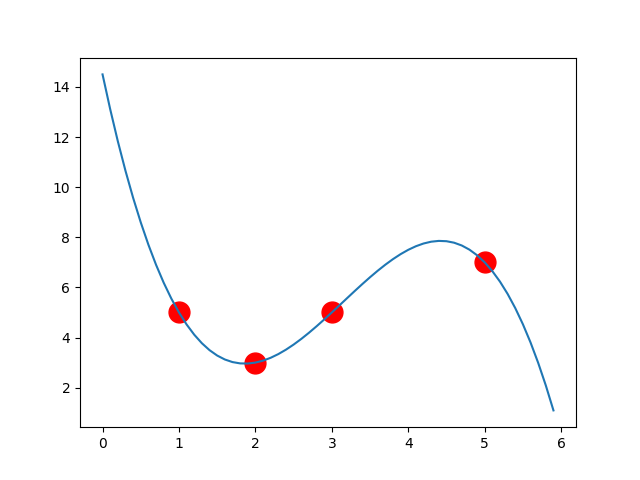
\includegraphics{5}
 		\section{Метод наименьших квадратов}
 		Метод наименьших квадратов (МНК) — математический метод, применяемый для решения различных задач, основанный на минимизации суммы квадратов отклонений некоторых функций от экспериментальных входных данных. Он может использоваться для «решения» переопределенных систем уравнений (когда количество уравнений превышает количество неизвестных), для поиска решения в случае обычных (не переопределенных) нелинейных систем уравнений, для аппроксимации точечных значений некоторой функции. МНК является одним из базовых методов регрессионного анализа для оценки неизвестных параметров регрессионных моделей по выборочным данным.@Wikipedia
 		
 		Чтож в применении к регрессионному анализу задачу МНК можно определить так:
 		Есть матрица $X$ и вектор $y$ нужно найти такую функцию $f(x)$ чтоы бы $\sum_i (f(x_i) - y_i)^2 \to min$ при том что $f(x) = f(x, \omega) = x_1 \omega_1 + x_2 \omega_2 \dots $ и по сути задача сводится к подбору $\omega$, и если рассматривать $\omega$ тоже как параметры то к $\min\limits_{ \omega} f(x, \omega)$. Чаще всего эту задачу решают методом градиентного спкска $\omega_{i + 1} = \omega_i + \alpha \bigtriangledown f(x, \omega)$.
 		
 		Пример использования(замечу что свободный коофицент не реализован так что если он нужен, добавлякься столбец полный 1):
 		\begin{verbatim}
 			from interpolation.linear_regression import LinearRegression
 			from interpolation.ploting import plot_result
 			
	 		lr = LinearRegression()
	 		x = [1, 2, 3, 4]
	 		y = [5, 6, 8, 10]
	 		x_with_one = list(map(lambda var_x: [var_x, 1], x))
	 		lr.fit(x_with_one, y, batchsize=1)
	 		plot_result(x, y, lambda x_1: lr.predict([[x_1, 1]]))
 		\end{verbatim}
 	На более сложных данных:
 	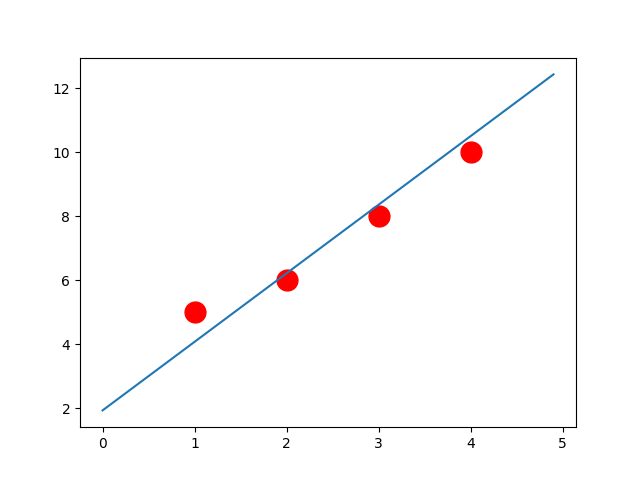
\includegraphics{6}
 	\begin{verbatim}
 		from interpolation.linear_regression import LinearRegression
 		from sklearn.datasets import make_regression
 		from interpolation.ploting import plot_result
 		
 		lr = LinearRegression()
 		x, y = make_regression(n_samples=100, n_features=1, noise=50, random_state=42)
 		x_with_one = list(map(lambda var_x: [var_x[0], 1], x))
 		lr.fit(x_with_one, y, batchsize=10)
 		plot_result(x, y, lambda x_1: lr.predict([[x_1, 1]]))
 	\end{verbatim}
 	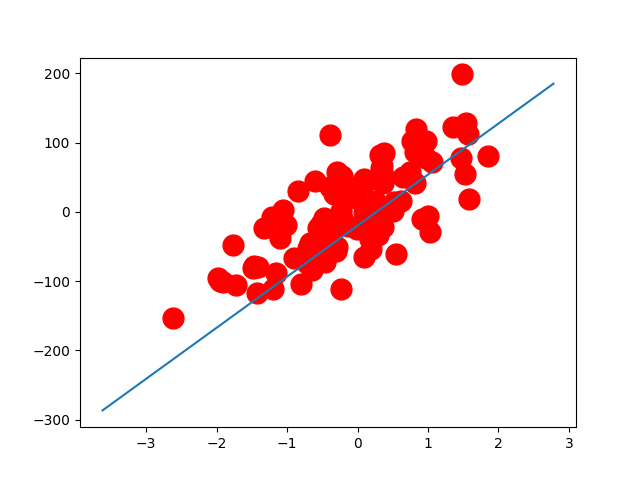
\includegraphics{7}
 	Сравним с sklearn:
 	\begin{verbatim}
 		from sklearn import linear_model
 		
 		lm = linear_model.LinearRegression()
 		lm.fit(x, y)
 		print(x)
 		plot_result(x, y, lambda x_1: lm.predict([[x_1]]))
 	\end{verbatim}
 	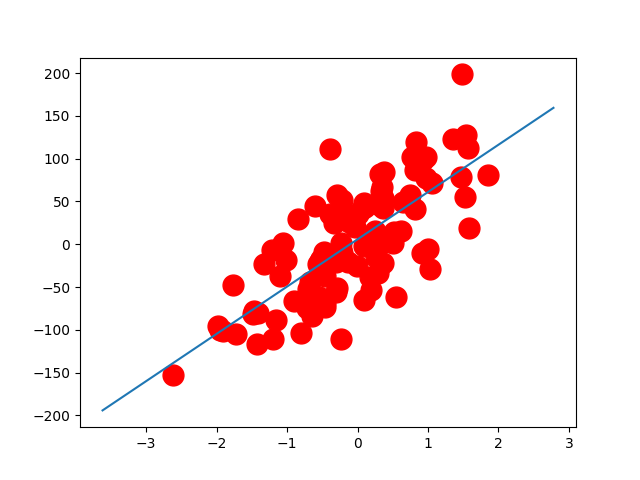
\includegraphics{8}
 		
 		
 \end{document}